\documentclass[a4paper,10.2pt,pdftex]{scrartcl}%NEU
\usepackage[T1]{fontenc}
\usepackage[utf8x]{inputenc} 
\usepackage[english, ngerman]{babel}
\usepackage[babel,german=swiss]{csquotes}
\usepackage{listings}
\usepackage{ltxtable} 
\usepackage{tabularx}
\usepackage{tabu}
\usepackage[final]{pdfpages}
\usepackage{graphicx}
\usepackage{url}
\usepackage{longtable}
\usepackage{wrapfig,lipsum,booktabs}
\usepackage{scrpage2} 
\usepackage{listings}
\pagestyle{scrheadings}
\automark{section}
%\usepackage{natbib}
%\usepackage[notocbib]{apacite}
\usepackage[top=3cm,bottom=3.5cm,left=3.5cm,right=3.5cm]{geometry} 

\usepackage{lmodern}

\DeclareOldFontCommand{\sc}{\normalfont\scshape}{\@nomath\sc}
\lstdefinelanguage{JavaScript}{
  keywords={typeof, new, true, false, catch, function, return, null, catch, switch, var, if, in, while, do, else, case, break},
  keywordstyle=\color{blue}\bfseries,
  ndkeywords={class, export, boolean, throw, implements, import, this},
  ndkeywordstyle=\color{darkgray}\bfseries,
  identifierstyle=\color{black},
  sensitive=false,
  comment=[l]{//},
  morecomment=[s]{/*}{*/},
  commentstyle=\color{purple}\ttfamily,
  stringstyle=\color{red}\ttfamily,
  morestring=[b]',
  morestring=[b]"
}

\lstset{
  basicstyle=\ttfamily,
}

%\usepackage{mathptmx}% Times (gut)
%\usepackage{beraserif}% Bera (wohl eher ungeeignet)
%\usepackage{mathpazo}% Palatino (gut!)
%\usepackage{bookman}% Bookman (etwas altert¸mlich)
%\usepackage{charter}% Charter (gut!) NEU
\usepackage{newcent}% Newcentury (gut)
%\usepackage{utopia}% Utopia (gut bis gut!)
%%%%% Ende Einfuegung

\usepackage[scaled]{helvet}%NEU
%\renewcommand{\sfdefault}{\rmdefault}%NEU

\usepackage[german]{varioref}

\usepackage{setspace}
\onehalfspacing
%\linespread{1.07}

\usepackage{ellipsis}

% .....

\usepackage[multiple]{footmisc}
%\usepackage[multiple,perpage]{footmisc}

\usepackage[alwaysadjust]{paralist}
\setlength{\pltopsep}{1ex}

%\deffootnote[1em]{1em}{1em}{\textsuperscript{\thefootnotemark\ }}

\usepackage[pdftex,
colorlinks=false, pdfborder={0 0 0},
bookmarksopen=true,
hyperfootnotes=false,
]{hyperref}
 

% Sicheres "Vgl.:" um Tippfehler zu vermeiden
\newcommand{\f}{\footnote}
\newcommand*{\VGL}{Vgl.:}
%\renewcommand{\opcittext}{a.~a.~O} 
%\renewcommand{\idemtext}{Ebenda} 
\newcommand{\first}[1]{\emph{#1}}
\newcommand{\q}[1]{\iflanguage{ngerman}{\flqq#1\frqq}{``#1''}}
\newcommand{\qq}[1]{\iflanguage{ngerman}{\frqq#1\flqq}{``#1''}}
\newcommand{\qs}[1]{\iflanguage{ngerman}{\flq#1\frq}{``#1''}}
\newcommand{\z}{\cite}
\newcommand{\e}{\emph}
%\newcommand{\c}{ \z}

% Korrekturanmerkungen am Rand (fett-kursiv)
\newcommand{\notiz}[1]{\marginline{\textbf{\textit{\footnotesize #1}}}}


%\hyphenation{Ge-schmacks-po-ren Ge-schmacks-po-re aus-schliess-lich Atmo-sph‰-re}

% BIBLATEX ?
%Infos

%\usepackage{biblatex}
%\include{natbib
\usepackage{bibgerm}
%\usepackage{opcit}
%\usepackage[notocbib]{apacite}
%\renewcommand{\opcittext}{a.a.O.}
%\renewcommand{\idemtext}{Ebenda}
\hyphenation{Wahr-nehm-ungs-}
\usepackage{xcolor}
%\pagecolor[HTML]{dedede}
\begin{document}

\begin{titlepage} 
 \begin{center} 
    \thispagestyle{empty}
  {\small  Hochschule Luzern \hfill Institut für Informatik   \\[.75ex]
\hrule 
\vspace{0.75ex}
WIPRO  \hfill Herbstsemester 2019\\  

%\hfill FS 2010
% \hfill Proseminar
}

%{\small }

\vspace{14ex}



{\LARGE Wirtschaftsprojekt}


\vspace{2ex}

%Anzahl Zeichen
{\large 20.\,Dezember\,2019}\\
\vspace{2ex}
%2\,500 Wörter

%\vspace{2ex}cv2.calcHist


\vspace{9ex}


{\huge\bfseries\textsf{Simulation und Visualisierung von \\[-1mm] Quantenkryptografie \\[5.5mm] }}

%\subtitle{}


\vspace{5ex}

%\vfill
Betreuungspersonen \\[2mm] Dr.\,Esther Hänggi \\ Dr.\,Halldór Janetzko\\[3mm]


\vspace{8ex}

{\Large Adrian Althaus \\[2mm] Fabian Meyer  \Large {}}

\vspace{8ex}

% {\large 17. M‰rz 2007}

 %\vspace{4ex}
 
%\vfill

\end{center}
\end{titlepage}

\vspace*{1ex}
\thispagestyle{plain}
\hspace*{-4.2cm}
\includegraphics[]{deckblatt.pdf} 
\newpage
\abstract{
\subsection*{Abstract}
Das Ziel dieser Arbeit besteht in der Simulation und Visualisierung des BB84-Protokolls. Dazu wurden zwei Applikationen entwickelt, zum einen ein Java-Backend, welches sich um die Simulation kümmert, und ein JavaScript-Frontend zur Visualisierung im Browser. Der Fokus des Backends liegt auf der korrekten Berechnung der Simulation und der sauberen Implementation mithilfe von komponentenbasierter Entwicklung. Der Schwerpunkt des Frontends liegt auf der Erklärungsfähigkeit, Interaktivität, Didaktik und Ästhetik. Die beiden Applikationen wurden auf dem Enterpriselab  der Hochschule Luzern deployt. Mit dem deployten Prototypen (Stand: 17.12). wurden Benutzertests durchgeführt, um ein Feedback zur Qualität der Applikation, insbesondere der Erklärungsfähigkeit, der Interaktion und der Visualisation einzuholen. Die Benutzertests fielen durchaus positiv aus, was als Projekterfolg gedeutet werden kann.} 
\newpage
\pdfbookmark{Inhalt}{toc}
\tableofcontents 
\newpage

\section{Problem, Fragestellung, Vision}
\subsection{Quantenkryptografie: Das BB84-Protokoll} 
In der Quantenverschlüsselung macht man sich Eigenschaften der Quantenphysik zunutze, um damit Informationen verschlüsseln zu können. Gleichzeitig ist es eine inhärente Eigenschaft eines quantenphysikalischen Systems, dass bei einem Messvorgang das System selbst gestört wird. Diese Eigenschaft wird ausgenutzt, um ein mögliches Abhören einer Botschaft detektieren zu können \cite{sicherheit}.

Eine Möglichkeit, Informationen mithilfe eines quantenphysikalischen Systems zu übertragen, ist die Polarisierung von Photonen. Dabei werden Photonen mithilfe geeigneter Gerätschaft polarisiert und dann durch einen Lichtwellenleiter verschickt. Am anderen Ende kann der Empfänger die Polarisation durch den Einsatz von optischen Geräten rekonstruieren und so die originale Botschaft wiederherstellen. 

Photonen können in 4 möglichen Zuständen polarisiert werden: 0°, 45°, 90° und 135°. Dabei stellen 0° und 90° gerade Polarisierungen dar und 45° und 135° diagonale Polarisierungen. Ein Bit kann nun in 2 möglichen Polarisierungen kodiert werden: 0 mit 0° oder 45° und 1 mit 90° oder 135°. Nur durch das Wissen sowohl über die Polarisierung als auch der richtigen Basis kann das korrekte Bit bestimmt werden.

Ist das Protokoll unter Einhaltung von gewöhnlichen Sicherheitsvorkehrungen erfolgreich durchgeführt worden, können der Sender und der Empfänger erfolgreich einen Schlüssel generieren, mit dem sie Informationen ähnlich einem one-time pad (symmetrisch) verschlüsseln und entschlüsseln können. 

Ein weiterer, wichtiger Vorteil von Quantenverschlüsselung im Gegensatz zur konventioneller (asymmetrischer) Verschlüsselung ist, dass die Etablierung des Schlüssels auf physikalischen Eigenschaften beruht und nicht auf mathematischen Berechnungen wie beispielsweise Hashfunktionen bei der asymmetrischen Verschlüsselung. Diese physikalischen Eigenschaften lassen sich auch mit erhöhtem Rechenaufwand nicht umgehen. Ebenso arbeitet man in der Quantenverschlüsselung weitgehend mit probabilistischen Verfahren. Aufgrund von quantenphysikalischen Eigenschaften ist ein Abfangen von Photonen zwar grundsätzlich feststellbar, aber letzten Endes lässt sich die Frage, ob Photonen abgehört wurden, nur mit einer bestimmten Wahrscheinlichkeit beantworten. 


\subsubsection{BB84 Protokoll}
Das BB84-Protokoll, benannt nach seinen Erfindern Charles Bennet und Gilles Brassard und seinem Veröffentlichungsjahr 1984, ist das bekannteste Protokoll zur Realisierung einer Quantenverschlüsselung. Es soll hier kurz beschrieben werden.

Der Einfachheit halber gehen wir von 3 Personen aus: Alice, welche die Nachricht verschickt, Bob, welche sie empfängt und Eve, welche die Nachricht abhören möchte.

\vspace{5mm}
Ablauf:
\begin{enumerate}
\item Alice erzeugt einen zufälligen, genügend langen Bitstring
\item  Diesen Bitstring enkodiert Alice, indem sie für jedes Bit eine zufällige Basis wählt (gerade oder diagonal) und damit jedes Photon polarisiert
\item  Die polarisierten Photonen schickt Alice mithilfe eines optischen Mediums (in der Regel ein Glasfaserkanal) an Bob
\item  Wenn Bob die Photonen erhält, misst er die Polarisierung jedes einzelnen Photons mithilfe seiner zufällig gewählten Basis (gerade oder diagonal) und dekodiert so den Bitstring
\item  Durchschnittlich sollte Bob zu 50\% die richtige Basis wählen und daher das korrekte Bit (0 oder 1) zu 50\% rekonstruieren können
\item  Bob befragt nun Alice (über einen authentisierten, öffentlichen Kanal) über die Basis jedes einzelnen Photons
\item Jedes Bit, welches durch eine falsch gewählte Basis bestimmt wurde, wird gekürzt. Das heisst der Schlüssel wird durchschnittlich 50\% kürzer
\item  Zum jetzigen Zeitpunkt sollten Alice und Bob denselben, identischen Bitstring besitzen, dieser wird auch \q{sifted key} genannt
\item  Alice und Bob können über einen authentisierten, öffentlichen Kanal ein Teil des Bitstrings miteinander vergleichen, um sicherzugehen, dass sie nicht abgehört wurden
\item  Dieser Teil wird dann verworfen. Der restliche Teil bildet den \q{shared secret key}
\item  Falls Eve die Nachricht abhören will, muss sie die Polarisierung der Photonen zwischen Alice und Bob messen. Auch Eve muss daher eine zufällig generierte Abfolge von Basen (gerade und diagonal) verwenden, um die Polarisation zu messen
\item  Wenn Eve eine falsche Basis gewählt hat, wird die Polarisierung des jeweiligen Photons zufälligerweise neu gesetzt
\item  Falls Eve alle Bits gemessen hat, sinkt die Wahrscheinlichkeit, dass Eve unentdeckt bleibt nach $n$ verglichenen Bits auf $(\frac{3}{4})^n$. Mithilfe von statistischen Tests kann überprüft werden, ob ein Mithörer die Photonen abgehört hat oder nicht
\item  Falls ein Mithörer vorhanden war, wird das Protokoll wiederholt oder die Übertragung abgebrochen
\item  Durch ein Absprechen können Alice und Bob eine andere Basenverteilung von geraden und diagonalen Basen als 50/50 benutzen. Dies führt zu längeren Schlüsseln bzw. weniger Kürzung
\end{enumerate}

\subsubsection{Kompromiss aus Simulation und Visualisierung des BB84-Protokolls}
Die Fragestellung, wie man einen solch komplexen Sachverhalt simulieren und gleichzeitig visualisieren könnte, bildete die Ausgangsstellung dieses Projektes. Von Anfang an gab es einen grossen Spielraum und Freiheit bei der Konzeption und Umsetzung. Da die beiden Autoren dieses Projektes einen anderen Background haben (Frontend bzw. Backend), kristallisierte sich langsam ein Konzept heraus, welches eine relativ klare Aufgabenteilung beinhaltete.

Für die Simulation bietet sich natürlich ein Backend an, bei welcher Performance und Robustheit oberste Priorität hat. Auf der anderen Seite kann die Visualisierung nur in einem Frontend sinnvoll verwirklicht werden, da hier mithilfe des Einsatz von Text, Bild und weiteren Medien die Thematik dem Benutzer erklärt werden kann.

Dies führte zu der Idee, eine Webapplikation zu programmieren, welche beide Anwendungen miteinander verbindet. Diese Verbindung führte zu einem bedingten Kompromiss: Das Backend generiert Daten für eine Simulation von quantenkryptografischer Verschlüsselung, bei welcher üblicherweise sehr grosse Datenmengen verarbeitet werden. Das Frontend hingegen muss den Sachverhalt möglichst einfach erklären können. Dazu sind keine grossen Datenmengen nötig. Die Daten werden für die Visualisierung über eine REST-Schnittstelle geladen. Insofern galt es eine Lösung zu finden, wie sich die beiden Anwenwendungsfälle -- didaktische Erklärung vs. produktiver Einsatz zur Generierung von Testdaten -- in Einklang bringen lassen.  

Dieser Kompromiss sollte erreicht werden, indem dem Benutzer trotzdem das Gefühl gegeben wird, dass hier sehr grosse Mengen von Daten verarbeitet werden können und der Benutzer einen Einblick in die Komplexität der Thematik erhält, indem die Komplexität auf ein Minimum reduziert wird. Gleichzeitig war klar, dass sich die physikalischen Komponenten so verhalten müssen, dass sie sowohl von einer REST-Schnittstelle angesprochen als auch in eine beliebige Applikation integriert werden sollen. 
 



\subsection{Schwerpunkte}
Durch die Unterteilung in Frontend und Backend und deren Zuweisung an eine Person ergeben sich in beiden Bereichen unterschiedliche Schwerpunkte. Beim Frontend geht es im Wesentlichen um die Darstellung der Simulation der einzelnen Schritte des BB84-Protokolls, um diesen Prozess für den Benutzer möglichst lehrreich, intuitiv, interaktiv und ästhetisch befriedigend visualisieren zu können. Dies beinhaltet die Repräsentation der einzelnen Komponenten der Simulation des BB84-Protokolls als UI-Elementen. Das Frontend soll vom User interaktiv bedienbar sein, um so die Erzeugung der Schlüssel der Quantenkryptografie auf geeignete Weise beeinflussen zu können.

Das Backend übernimmt die Abbildung der physikalischen Vorgänge des BB84-Protokolls als einzelne Komponenten, welche über Schnittstellen miteinander verbunden sind und welche zu einem späteren Zeitpunkt mühelos erweitert, ausgetauscht und angepasst werden können. Die Simulation soll schlussendlich über eine API von aussen benutzbar, konfigurierbar und abgreifbar sein, mit einem Bytestream als Output.

Unabhängig von der Umsetzung und der Arbeitsteilung bildet ein Schwerpunkt die Erlangung der nötigen physikalischen Kenntnisse, die für ein vertieftes Verständnis des BB84-Protokolls erforderlich sind.

\section{Stand der Praxis}
\subsection{Informationsvisualiserung}
In den letzten Jahren haben sich die Möglichkeiten in der Datenvisualisierung rasant verändert. Gleichzeitig findet eine Verschiebung von statischer Berichterstattung mit Text und Bild zu dynamischen, interaktiven Multimediaformen statt.

Beispielsweise besitzt die Onlineausgabe der \emph{New York Times} seit dem Jahr 2014 eine neue Sparte namens \q{The Upshot}\footnote{\url{https://www.nytimes.com/section/upshot}}, auf welcher Artikel veröffentlicht werden, die politische, wirtschaftliche oder gesellschaftliche Themen durch den Einsatz von Techniken des Datascience und Datenvisualierung ergänzen, sogenanntes \q{data-driven storytelling}. Diese Artikel sind dynamisch und interaktiv; der Benutzer kann die Daten manipulieren und so direkt in die Visualisierung eingreifen.

Möglich macht dies Fortschritte nicht nur in der Produktion leistungsfähigerer Computerhardware, sondern auch die Entwicklung von immer leistungsfähigerer Browsersoftware. Dabei findet eine stetige Verschiebung von Rendering auf der Serverseite zum Rendering auf der Clientseite statt. Wo früher grosse Mengen von Daten nur auf hochspezialiserten Computer berechnet und visualisiert werden konnten, kann dies heutzutage auch auf einem PC im Browser realisiert werden. Daher erstaunt es nicht, dass auch spezialisierte Datenvisualierungsbibliotheken, wie D3 für die clientseitige Scriptsprache JavaScript zur Verfügung stehen.

\subsection{Explorable Explainables}
In den letzten Jahren sind auch einige Tools, Frameworks, Markupsprachen oder Bibliotheken erschienen, welche sich darauf spezialisieren, Techniken der Datenvisualisierung zu benutzen, um so dynamischen, interaktiven und multimedialem content zu erzeugen. Diese unterscheiden sich jedoch gross in Bezug auf die Voraussetzungen des angesprochenen Benutzers (Informatik-Hintergrund oder Autor bei einer Zeitung) oder der Domäne (spezialiserte Software oder allgemein einsatzfähig).

Diese Art von Software, welche Berichterstattung mit interaktiven Techniken der Datenvisualierung kombiniert und deren Resultate, wird als \emph{Explorable Explainables} bezeichnet. Die Abgrenzung zu anderer Software ist nicht ganz eindeutig, beispielsweise kann auch Project Jupyter verwendet werden, um Daten interaktiv zu visualisieren und dies einer grossen Audienz zugänglich zu machen. Jedoch verlangen Jupyter notebooks sehr viel Vorkentnisse in der Informatik und sind daher auf eine bestimmte Zielgruppe beschränkt. 
\subsection{Idyll}
Eine dieser Markupsprachen ist Idyll \footnote{\url{https://idyll-lang.org}}, welche die Erzeugung interaktiver Dokumente mit der Markupsprache Markdown verbindet. Idyll stellt eine Reihe von UI-Komponenten zur Verfügung, mit welchen sich einerseits Inhalte wie Text, Bild und Visualisierungen darstellen lassen, als auch Komponenten wie Regler, Eingabefelder und weitere, um Daten zu manipulieren.

Idyll selbst basiert auf der UI-Bibliothek React \footnote{\url{https://reactjs.org}}, einem JavaScript Frontend-Framework, welches anfänglich von Facebook entwickelt wurde und im Jahr 2013 als open-source Projekt der Öffentlichkeit zugänglich gemacht wurde. Die Philosophie von React beruht einerseits auf der Entwicklung von Komponenten mit Schnittstellen, die wiederverwendet werden können und andererseits auf der reaktiven Programmierung, ein relatives neues Programmierparadigma, welches Zustände und Änderungen einzig und allein auf Datenflüsse zurückführt. React eignet sich insbesonders um single-page Applications (SPAs) zu erzeugen. Dabei wird bei einem Seitenaufruf nur eine leere Hülle aus HTML geladen und der gesamte Content wird beim Client im Browser dynamisch durch JavaScript erzeugt (Clientside Rendering).

Idyll verknüpft die einfache Herstellung von Komponenten von React mit dem simplen Markupsyntax von Markdown, mit welchem sich rasch einfache Dokumente schreiben lässt. Ähnlich wie bei LaTeX, wird bei Markdown Inhalt und Struktur gegenüber Layout getrennt. Das Layout kann einfach mit einer CSS-Datei gesteuert werden.

In Idyll wird also der einfache Syntax zum Schreiben von Texten mit Markdown mit dem System zur Erzeugung von Komponenten von React verknüpft. Bei der Kompilation werden gewöhnliche JavaScript-, HTML- und CSS-Dateien erzeugt, welche statisch auf einem Server abgelegt werden können.
\newpage
\subsection{Vergleichbare Projekte}
Es existieren wenige Projekte, welche sich zum Ziel gemacht haben, das BB84-Protokoll oder Quantenverschlüsselung allgemein zu simulieren und visualisieren. 

Eines davon ist von Fred Henle aus dem Jahr 2008\footnote{\url{http://fredhenle.net/bb84/demo.php}}, welches das BB84-Protokoll auf eine spielerische Weise erklärt. Wie man rasch erkennt, ist es schon ein bisschen in die Jahre gekommen und entspricht nicht mehr dem Verständnis und Aussehen moderner Webseiten. Trotzdem ist es auf der englischsprachigen Wikipediaseite \footnote{\url{https://en.wikipedia.org/wiki/Quantum_key_distribution}} zu \emph{Quantum key distribution} aufgelistet.

Ein nennenswertes Beispiel ist auch der \emph{Quantum Computing Playground} \footnote{\url{http://www.quantumplayground.net/\#/home}}, mit welchem sich die Programmierung von Qubits mithilfe von Quantengates simulieren lässt. Obwohl sehr leistungsfähig (die Grafiken werden mit WebGL gerendert) und wissenschaftlich exakt, ist es nicht der Anspruch dieser Seite, eine solch komplexe Thematik auf einfache und verständliche Art und Weise erklären zu wollen.

Eine erschöpfende Liste von Software, welche sich primär mit Quantumcomputing befasst oder diese simuliert findet man auf Quantiki\footnote{\url{https://www.quantiki.org/wiki/list-qc-simulators}}, dem bekanntesten Informationsportal zu allen Themen der Quanteninformationstheorie und deren Anwendungen.
% Backend: Event getrieben vs Simulation getrieben. 

\subsection{Modularisierung}
% Backend: Event getrieben vs Simulation getrieben. 
Modularisierung ist ein grundlegendes Prinzip der Softwaretechnik. Sie hilft bei der Komplexitätsreduktion und erhöht die Flexibilität von Software. Unterteil man Software in verschiedene Module, so geschieht dies nach gängigen Kriterien wie minimale Schnittstellen, maximale Bindung, minimale Kopplung oder Testbarkeit. Im Falle einer Simulation mit physikalischen Komponenten liegt es nahe, die einzelnen Komponenten als in sich geschlossene Module zu betrachten. In Java geschieht dies auf technischer Ebene mit Interfaces. Damit eine Klasse zum Modul wird, muss sie richtig konzipiert sein. Unterstützend wirken Pakete und JARs, die aber keine Zugriffskontrolle über eine Schnittstelle kennen. Vor Java 9 war eine echte Modularisierung nur mit \emph{Open Services Gateway} (OSGi) möglich, welche aber nicht Teil des Standardumfangs von Java ist \cite[S. 32f]{modul}

\subsubsection{Modularisierung mit Java 9} 
Mit dem lange erwarteten Projekt \emph{Jigsaw} ist nun eine explizite Erstellung von Modulen möglich. Sie können aus einem oder mehreren Paketen bestehen, und ihre Sichtbarkeiten und Abhängigkeiten sind klar definiert. So lassen sich gleichsam verschachtelte Modulabhängigkeiten und transitive Abhängigkeiten verwirklichen. Ein Modul besteht aus einem Namen, einer Schnittstelle und natürlich der Implementierung. Im Zuge von Jigsaw wurde auch das JDK in eine Vielzahl von Modulen aufgeteilt \cite[S. 863]{inden}. 

\begin{table}
\hspace{1cm}
\begin{tabular}{ll}
\texttt{exports} & Öffentlich zugänglich gemachte Pakete \\
\texttt{requires} & Liste importierbarer Module \\
\texttt{uses / provides} & Benötigter und angebotener \emph{service} \\
\texttt{opens} & Zugriff über Reflection erlauben
\end{tabular} 
\caption{Jigsaw Keywords}
\end{table}

Skalierbarkeit der Java-Plattform, Erhöhung der Sicherheit, Start-up-Performance, Unterstüztung beim Entwurf modularer und gut wartbarer Anwendungen und Bibliotheken gelten als allgemeine Ziel der Modularisierung und der komponentenbasierten Entwicklung. Mit dem Projekt Jigsaw ist Java 9 ein wichtiger Schritt in die richtige Richtung gelungen. So lohnt es sich, bei der Entwicklung von grösseren Projekte auf diese Technologie zu setzen, während die Migration von älteren Versionen mit verwendeten Modulen mit gewissen Problemen verbunden sein kann\cite[Kap. 15.4.2]{inden}. 


\section{Ideen und Konzepte}
Aus der Aufgabenstellung geht hervor, dass sich das Projekt zum einen gewisse didaktische Anforderungen erfüllen muss, zum anderen die Einbettung in bestehende Systeme am Departement für Informatik zu berücksichtigen hat. Insofern wurden Ansätze einer monolithischen Applikation bereits bei den ersten Überlegungen verworfen. Vielmehr hatte sich rasch herauskristallisiert, dass die unterschiedlichen Anwendungsfälle am besten mit einem modularen Kernsystem abgedeckt werden, die dann entweder in einem diaktischen Kontext als Webapplikation, oder dann eben im produktivem Einsatz beispielsweise als CLI-Tool eingebunden werden. Dadurch lässt sich das Projekt zudem in ein Frontend und Backend einteilen, für die dann -- abhängig von den jeweiligen Präferenzen --  je einer der beiden Projektpartner zugewiesen werden können. Zum Projektstart hat man sich auf eine Modellierung geeinigt, die das BB84-Protokoll physikalisch in einer Webapplikation abbildet, wobei es zu der jeweiligen physikalischen Komponente je eine Entsprechung im Frontend und Backend gibt, die miteinander interagieren. Der Ablauf des BB84-Protokolls wird somit in Teilschritte gegliedert, die unabhängig voneinander atomar ausgeführt werden können. Bei jedem dieser Teilschritte wird die REST-Schnittstelle mit den benötigten Parametern angesteuert. Das Backend arbeitet damit stateless. 

\subsection{Alternative Ideen}
Die offene Aufgabenstellung und die Zielsetzung lassen viele Freiheiten bei der Konzeption des Projekts zu.

Da die beiden Autoren jedoch unterschiedliche Ausrichtungen, Fähigkeiten und Interessen besitzen, hat sich ein Konzept angeboten, welche auf der Frontendseite die Visualierung und auf der Backendseite die Logik umsetzt. Für das Backend sollen Module entwickelt werden, die in unterschiedlichen Kontexten eingebunden werden können. Dies erschien als die sinnvollste Lösung für die beiden unterschiedlichen Anwendungszwecke. Die Kombination aus Idyll und Java-Backend musste sich erst herauskristallisieren. Für Java sprach die Unterstützung von Modularisierung ebenso wie der Aspekt der Performance. Darüber hinaus wird Java an der Hochschule Luzern unterrichtet. Idyll machte mit Blick auf die Idee eines interaktiven Papers einen überzeugenden Eindruck. Dennoch standen Sprachen wie Python oder Kotlin als Backendlösung zur Debatte. 

Hinsichtlich der Kommunikation zwischen Frontend und Backend war es lange nicht ganz eindeutig, inwiefern das Backend Kenntnisse über den Zustand des Frontends haben sollte. Versuchsweise wurde deshalb für die Zwischenspeicherung von berechnetetn Werten auf dem Server eine Unterstützung für Sessions eingebaut. Das Frontend beinhaltete in einer früheren Version einen Settings-Button, der Parameter, die bei mindestens zwei unterschiedlichen physikalischen Komponenten benötigt werden, an den Server für eine Ablage in der Session sendet. Im weiteren Projektverlauf wurde dieser Ansatz verworfen, weil sich die Anzahl Parameter wie auch die Datengrösse der Payloads im jeweiligen Requests in Grenzen hielt. Die Verbindung einer REST-Schnittstelle und Sessions erschien dann quasi als Antipattern, da REST für ein zustandsloses Paradigma steht. Ein zustandsloses Backend macht grundsätzlich Sinn, da sich atomare Ausführungseinheiten besser parallelisieren oder gar auslagern lassen, etwa in eine Cloud als Function-as-a-Service. Die Logik kann dann problemlos ans Frontend ausgelagert werden. Wenn das Zusammenspiel mit dem Frontend  aus Sicht des Backends zustandslos funktionert, wird es dies bei der Einbindung der Komponenten in einen anderen Kontexten auch tun. 

\section{Methoden}
\subsection{Vorgehensmodell}
Aufgrund der Aufgabenstellung empfiehlt sich ein hybrides Vorgehensmodell nach SoDA. Ein Wasserfallmodell ist aus dem einfachen Grund ausgeschlossen, dass zum Zeitpunkt des Projektstarts der genaue Projektumfang noch nicht vorlag. Das Minimalziel liegt in der Umsetzung der Minimalanforderung, i.e. ein Schulbeispiel des BB84-Prototkolls. Die weiteren Punkte während der Projektverlaufs fortwährend festgelegt. Die Abstände zwischen den Treffen mit den Auftraggebern erlaubt ein agiles Vorgehen. Der primäre Milestone bestand in der Abnahme des Testates in der Semesterwoche 10, wo es die Erreichung der minimalen Ziele unter Beweis zu stellen galt.

\subsection{Frontend: Benutzertests}
Zur Evaliation des Frontends wurde ein high-fidelity Prototyp (Stand: 17.12.2019) auf dem Enterpriselab deployt. Dann wurden Informationen an Bekannte ausgegeben mit der Bitte, den Prototypen zu testen und das Formular mit den Fragen (auf Google forms) auszufüllen. Es wurden bewusst Personen aus verschiedenen Altersklassen und Berufen ausgewählt, da es ja gerade das Ziel des Frontends ist, den Sachverhalt zu erklären.

Es wurden Remote Usertests durchgeführt, das heisst alle Benutzer konnten den Prototypen von zuhause aus in Ruhe anschauen und testen. Es wurden zuerst allgemeine Fragen zu Geschlecht und Alter und je eine Frage zum Wissenstand in Physik respektive Informatik gestellt. Die Fragen zum Wissenstand wurden quantitativ  mit Werten von 1 bis 6 beantwortet. Dies diente als Warm-up für die Benutzer und um nötige demografische Informationen und Anhaltspunkte zum Wissenshintergrund der Testpersonen zu erlangen.

Dann wurden je 4 Fragen zu den Bereichen Erklärung (Erklärungsfähigkeit), Interaktion und Visualisierung gestellt. Bei jedem Bereich wurde zuerst eine allgemeine Frage zum Eindruck davon quantitativ gestellt (1 bis 6), dann je eine qualitative Frage, was man besonders gut fand, je eine qualitative Frage, was man besonders schlecht fand und wieder eine quantitative Frage (1 bis 6) zu einem bestimmten Komponenten. Damit erfolgt wieder zuerst ein warm-up mit einer einfacheren, allgemeinen Frage.

Zum Schluss konnten die Benutzer frei ihre Gedanken als Anmerkungen, Kritik, Wünsche und offene Fragen. Damit konnte man alle Informationen abfangen, zu denen vorher keine Fragen gestellt worden sind.

Die Evaluierung der Benutzerumfrage fliess so gut es ging noch in die Weiterentwicklung der Applikation (insbesondere des Frontends) mit ein. Die Erkenntnisse der Resultate sind im Kapitel 6 festgehalten und der Fragebogen mit Antworten im Anhang.

\subsection{Testing Backend}
Im Backend sind im test-package für jede Komponente JUnit-Tests enthalten, welche die korrekte Berechnung der entsprechenden Aufrufe sicherstellen sollen. Die Tests enthalten in aller Regel bestimmte Strings aus Bits, Basen oder Polarisierung, für die eine bestimmte Komponente den jeweiligen Wert berechnen muss.\footnote{Die Unit-Tests lassen sich in der Konsole im Verzeichnis vom Backend mit \\ \texttt{./gradlew test} ausführen.}


\section{Realisierung}
Die Aufgabenstellung verlangt eine Art Zweiteilung der Programmierarbeiten. Die Umsetzung der physikalischen Komponenten ist zunächst einmal unabhängig vom Einsatzzweck. Bei den beiden Anwendungsfällen aber werden sie auf unterschiedliche Weisen angesprochen. Bei der Vermittlung des BB84-Protokolls an interessierten Personen kommt ein interaktives Webfrontend zum Zuge, das über eine REST-Schnittstelle mit dem Java-Backend kommuniziert. Die eigentlichen Komponenten können als Java-Kompontenten angesprochen werden. 


\subsection{Frontend}
Das Frontend wurde mithilfe von Idyll und React umgesetzt. Die Grundstruktur eines idyll-Projektes besteht aus einem index.idyll file und einem Ordner mit allen Komponenten. Das index.idyll File ist vergleichbar mit einem HTML-file, welches für die Struktur des Dokumentes zuständig ist. In dieses file wird dann der gesamte Text und alle Komponenten eingebunden.
\subsubsection{Verwendete Idyll-Komponenten}
Idyll bringt eine Reihe von Komponenten mit, die jedoch alle ziemlich simpel sind und von welchen nicht gross Gebrauch gemacht wurde. Einzige Ausnahmen sind:

\begin{tabularx}{\textwidth}{p{2.5cm}p{8.5cm}}
Header & Der header der Webseite, mit allen wichtigen Informationen.\\
var & Eine Input-Komponente, mit der man eine Variable definieren kann. \\
fullWidth & Eine Komponente, welche als Wrapper benutzt wird, um den inneren Komponenten auf die ganze Seitenbreite zu rendern. \\
Equation & Eine Komponente, welche es ermöglicht LaTeX-Syntax direkt im index.idyll-File zu schreiben. \\
Display & Eine Komponente, welche den Wert einer Variable anzeigt, mit zusätzlichen Möglichkeiten der Formatierung.
\end{tabularx}

\subsubsection{Verwendete npm packages}
\begin{tabularx}{\textwidth}{p{3cm}p{8.5cm}}
react-arrow &  Ein package, welches eine Komponente ausgibt, die einen Pfeil als canvas-Element rendert. \\
react-anime &  Ein package, welches einen Wrapper um die JavaScript-Bibliothek animejs bildet. Damit lassen sich Animationen generieren, indem man für verschiedene Keyframes Werte eines bestimmten properties eingibt. \\
react-emoji-render &  Ein package, mit welchem sich einfach ein emoji darstellen läst. \\
react-rough &  Ein package, welches einen Wrapper um die JavaScript-Bibliothek roughjs bildet, mit der man Grafiken als canvas oder svg rendern kann, die einen handgemalten Stil besitzen. Sämtliche Grafiken in der Applikation wurden mit diesem package erstellt. \\
react-slider&  Ein package, mit welchem sich einfach ein Regler rendern lässt und bei dem man alle grafischen  Details per css genau steuern kann. Dieses package wurde verwendet um alle Regler im Dokument zu erstellen. \\
rodal&  Ein package, welches ein Modal (ein kleines Fenster, welches alles andere im Hintergrund verblasst)  rendert.
\end{tabularx}

\subsubsection{Arten von Komponenten}
\begin{tabularx}{\textwidth}{p{3cm}p{8.5cm}} 
Visuelle Komponenten &  Sind Komponenten, die Sachverhalte visuell darstellen, um sie so dem Benutzer veranschaulicht erklären zu können. \\
Logik-Komponenten & Sind Komponenten, die für die Logik des Frontends gebraucht werden, um den Ablauf des Algorithmus darstellen zu können. Sie sind entweder mit dem backend via der REST-API verbunden oder benutzen eine interne Logik, welche nur für das frontend von Bedeutung ist. \\
Input-Komponenten & Sind Komponenten, die der Benutzer bedienen kann, um den Programmablauf zu steuern.
\end{tabularx}

\subsubsection{Erstellte Komponenten} 
\begin{description}
\item[SystemOverview] Eine visuelle Komponente, die dazu dient, dem Benutzer schon früh im Dokument eine Übersicht über das BB84-Protokoll zu geben und ihm die Möglichkeit zu geben, wichtige Einstellungen der Simulation festlegen zu können. Sie zeigt die drei Teilnehmer des Algorithmus, Alice, Bob und Eve, sowie die zwei Übertragungskanälen samt den einstellbaren Parameter.
\begin{figure}[h]
	\centering
  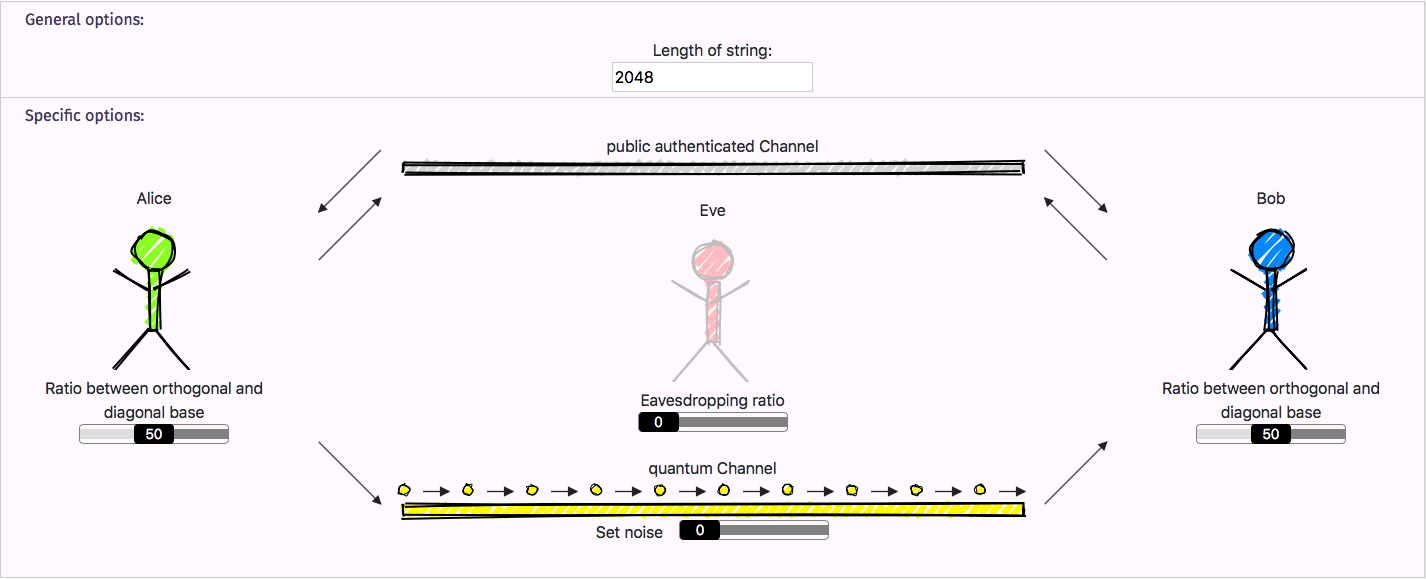
\includegraphics[width=\textwidth]{graphics/component_system_overview.png}
	\caption{System overview}
\end{figure}
\item[ButtonAliceStart] Eine Logik-Komponente, welche einen Button rendert, der den Algorithmus startet. Dabei wird die \texttt{strLength} zusammen mit \texttt{AliceProb} per POST-Methode an das Backend geschickt, um damit Alices Bitstring und ihre Base zu berechnen. Als Antwort kommt dann der Bitstring und die Base zurück.
\begin{figure}[h]
	\centering
  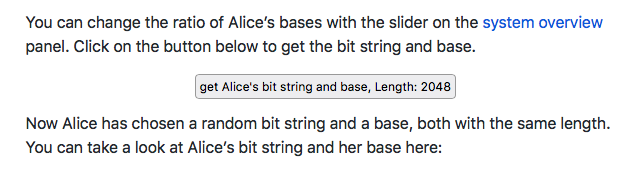
\includegraphics[width=\textwidth]{graphics/component_button_alice_start.png}
	\caption{System overview}
\end{figure}
\item[PhotonGridDouble] Eine visuelle Komponente, welche zwei Strings entgegennimmt und diese rendert als zwei Raster von einzelnen Symbolen. Der Hintergrund des Rasters kann bei Bedarf gefärbt werden (was am Schluss auch gemacht wird). Diese Komponente wird benutzt um zwei Strings (Bitstring oder Base) darzustellen. Per Klick auf das Raster öffnet sich ein Modal, welches den String in einem quadratischen Fenster darstellt (Komponente ScrollBox). 
\begin{figure}[h]
	\centering
  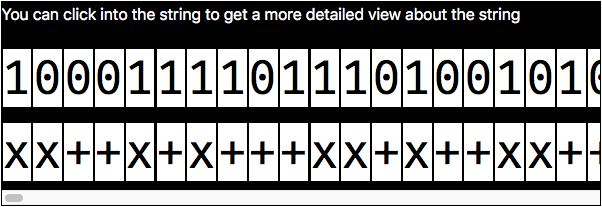
\includegraphics[width=0.5\textwidth]{graphics/component_photon_grid_double.png}
	\caption{Photon grid double}
\end{figure} 
\item[scrollBox] Eine visuelle Komponente, welche einen String in einem quadratischen Fenster darstellt. Es besitzt einen Slider, mit dem man die Schriftgrösse des Keys anpassen kann. Wird die Schriftgrösse zu klein, wechselt die Darstellung des Schlüssels von Text zu einem Bitmuster. Es existiert eine kleine Legende, welche die Farben des Bitmusters erklärt.
\begin{figure}[h]
	\centering
  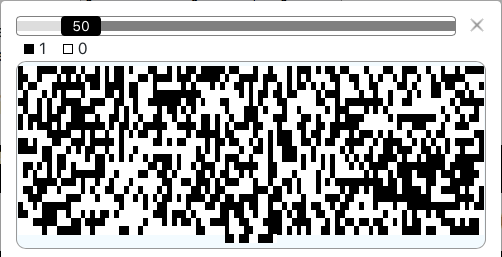
\includegraphics[width=0.5\textwidth]{graphics/component_scroll_box.png}
	\caption{Scroll Box}
\end{figure}
\item[InformationBox] Eine visuelle Komponente, welche eine Tabelle rendert, die den für das Verständnis wichtigen Zusammenhang zwischen Bitstring, Base und resultierende Polarisation veranschaulicht.
\begin{figure}[h]
	\centering
  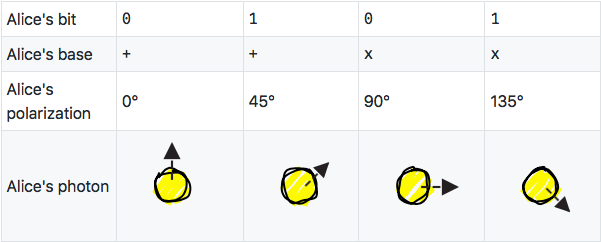
\includegraphics[width=0.5\textwidth]{graphics/component_information_box.png}
	\caption{Information Box}
\end{figure}
\item[SimpleSlider] Eine kleine Input-Komponente, welche nur einen Regler rendert, der genau ein property beeinflusst. 
\begin{figure}[h]
	\centering
  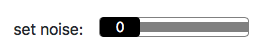
\includegraphics[width=0.4\textwidth]{graphics/component_simple_slider.png}
	\caption{Simple slider}
\end{figure}
\item[ButtonEmitPhotons] Eine Logik-Komponente, welche einen Button rendert, der den Algorithmus weiterführt. Damit wird aus dem Bitstring und der Base von Alice ein String von Polarisationen berechnet. Der Bitstring und die Base werden wieder per POST-methode an das backend geschickt und als Antwort kommt ein String von Polarisationen für Bob zurück.
\begin{figure}[h]
	\centering
  
\includegraphics[width=0.4\textwidth]{graphics/component_button_emit_photons.png}
	\caption{ButtonEmitPhotons}
\end{figure}
\item[ShowHide] Eine kleine Logik-Komponente, welche als Wrapper dazu dient eine innere Komponente mithilfe einer Bedingung ein- oder ausblenden zu können. So können zum Beispiel Visualisierungen oder Animationen nach Bedarf eingeblendet werden.
\item[AnimationEmit] Eine visuelle Komponente, welche darstellt, dass Photonen von Alice zu Bob geschickt werden
\begin{figure}[h]
	\centering
  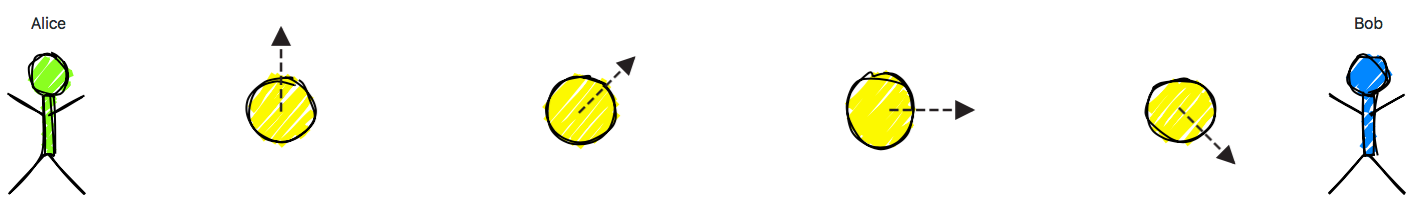
\includegraphics[width=\textwidth]{graphics/component_animation_emit.png}
	\caption{AnimationEmit}
\end{figure}
\item[ButtonBobBase] Eine Logik-Komponente, welche durch die Stringlänge und die Wahrscheinlichkeit der Basenverteilung von Bob eine Base für Bob berechnet. Die Stringlänge und die Wahrscheinlichkeitsverteilung werden per POST-methode an das backend geschickt, welches als Antwort eine Base für Bob zurückschickt. 
\begin{figure}[h]
	\centering
  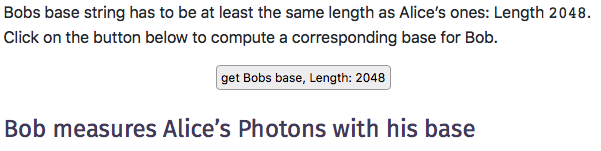
\includegraphics[width=0.8\textwidth]{graphics/component_button_bob_base.png}
	\caption{ButtonBobBase}
\end{figure}
\end{description}
\newpage
\subsection{Starten des Frontends}
Da das Frontend auf JavaScript läuft, benötigt es den JavaScript package manager npm. Dieser kann mit \texttt{npm install npm@latest -g} installiert werden. Dann müssen im Verzeichnis des Frontends alle nötigen packages installiert werden: \texttt{cd path/to/wipro-v1 \&\& npm install}. Schliesslich kann das Frontend gestartet werden mit dem Befehl \texttt{idyll}.

\subsection{Physikalische Komponenten}
Im Backend sind die physikalischen Komponenten verwirklicht, welche je durch eine eigene Klasse repräsentiert werden. Die Anzahl Komponenten wie auch deren Attribute sind gegeben durch die erreichte Funktionalität in der Umsetzung des BB84-Protokolls. Den Komponenten im Backend entspricht in der Regel eine Komponente im Frontend, jedoch kann ein Schritt in der Durchführung mehrere Komponente involvieren. Folgende Komponenten wurden umgesetzt:
\begin{description} 
\item[RandomBitString] Generiert einen Bitstring der Länge n \\
\begin{tabular}{p{3cm}p{9cm}}
stringLength & Länge des Bitstrings \\
prob & Wahrscheinlichkeit von 0 oder 1 \\
\end{tabular}
\item[RandomBase]  Generiert eine zufällige Basis \\
\begin{tabular}{p{3cm}p{7.5cm}}
n & Länge der Base \\    
prob & Wahrscheinlichkeit von Rückgabewert orthogonal im Verhältnis zu diagonal
\end{tabular} 
\item[PhotonEmitter] Schickt eine Reihe von Photonen  \\
\begin{tabular}{p{3cm}p{9cm}}
base & Base \\
str & bitString \\  
\end{tabular}
\item[PhotonReceiver]
Diese Komponente repräsentiert Bob, der einen Photonenstring empfängt.  \\
\begin{tabular}{p{3cm}p{7.5cm}}
photons & Photon String   \\
base  & String mit Basen  \\
noise &  Noise String, 0 - 100  \% \\ 
eavesdropping  & Anteil an Eavesdropping 
\end{tabular} 
\item[QuantumChannel] 
Diese Komponente repräsentiert den Übertragungskanal. \\
\begin{tabular}{p{3cm}p{7.5cm}}
Noise  & Polarisierung verändert sich, 0 - 100\% \\
Eavesdropping & Polarisierung verändert sich, 0 - 100\% \\
\end{tabular} 
\item[BaseComparator] Diese Komponente vergleicht zwei Basenstrings miteinander \\  \begin{tabular}{p{3cm}p{9cm}}
Base1 & Base String 1   \\
Base2 & Base String 2  
\end{tabular}
\item[KeyShortener] 
Diese Komponente vergleicht die Basen von Alice und Bob und simuliert damit die Absprache über den öffentlichen Kanal. Anhand der Bitstrings von Alice und Bob werden damit zwei unterschiedliche Bitstrings zurückgegeben, die jeweils einen Underscore an allen Stellen enthalten, an der sich die entsprechenden Stellen in den beiden Basen unterscheiden. 
\\
\begin{tabular}{p{3cm}p{7.5cm}}
base1  & Basis von Alice \\
base2  & Basis von Bob \\
string\_alice &  Bitstring von Alice \\
string\_bob & Bitstring von Bob \\ 
state\_string & Spezieller Statusstring vom Frontend, der die Information über Noise und Eavesdropping an den jeweiligen Stellen für die Visualisierung enthält und der bei jeder Abweichung der Basen gekürzt werden muss \\
\end{tabular} 
\item[KeyComparator] 
Diese Komponente überprüft die Bitstrings von Alice und Bob und überprüft anhand eines prozentualen Werts, wie hoch der Anteil sein soll, der überprüft und danach verworfen werden soll. \\
\begin{tabular}{p{3cm}p{7.5cm}}
restStringAlice  & Polarisierung verändert sich, 0 - 100\% \\
restStringBob & Polarisierung verändert sich, 0 - 100\% \\
colorString & String, der spezifisch für das Frontend mitvearbeitet wird und die Statusinformationen zu den Photonen enthält, der mit der Kürzung ebenfalls gestutzt werden muss. 
\end{tabular} 
\end{description}
\subsection{Modularisierung}
Der Grad an Modularisierung ist bei dieser Art von Realisierung weniger hoch ausgefallen als ursprünglich angedacht. Während des Projektverlaufs hat sich der erste Anwendungsfall -- die interaktive Einführung in die Thematik -- als deutlich relevanter herausgestellt. Nach dem Entscheid, die gesamte Kommunikation beider Teilprojekte über eine REST-Schnittstelle abzuwickeln, hat sich das stateless-Prinzip durchgesetzt. Alle Aufrufe sind atomar. Auch bei der direkten Einbindung der Komponenten in weitere Java-Klassen scheinen die separaten, statischen Aufrufe zu genügen. Damit wurden auch der Ansatz, Einstellungen etc. in Sessions zu hinterlegen, verworfen. Dies bedeutet demnach eine vollständige Beschränkung auf \texttt{static}-Methoden, die sich bekanntermassen schlecht über Interfaces managen lassen. Eine statische Methode  muss in einem Interface ausimplementiert werden und lässt sich danach nicht mehr überschreiben. 

Alle physikalischen Modelle befinden sich in einem separaten Package, besitzen aber keinen Konstruktor und sind aus den genannten Gründen \emph{nicht} über Interfaces aufrufbar. Und so macht es auch wenig Sinn, Jigsaw einzusetzen, zumal es auch keine komplizierten Abhängigkeiten und Verschachtelungen von Modulen gibt. Zudem haben sich erste Tests mit Java 9 mit der verwendeten Konfiguration von Gradle gebissen.  

Im Backend befindet sich die Klasse \texttt{MessagePackClient}, welche die Einbindung der Komponente unabhängig von der Webapplikation zeigen soll. In ihr ist MessagePack\footnote{\url{https://msgpack.org/}} eingebaut, was ein Serialisierungstool ist, das JSON-ähnliche Outputs liefert. Es untersützt alle möglichen Datentypen, insbesondere auch Byte-Arrays. Die Datei zeigt einen möglichen Aufruf der Komponenten, wobei mit \texttt{RateLimiter} aus dem Guava-Projekt eine Throttling-Möglichkeit besteht, sodass die Photonen einzeln in einem bestimmten Intervall verarbeitet werden können. 

\subsection{Webserver im Backend}
\begin{figure}
\includegraphics[width=\textwidth]{graphics/architecture.pdf}
\caption{Architekturübersicht}
\end{figure}

Im Backend residiert ein Tomcat-Server. Bei der lokalen Entwicklung wird er als EmbeddedTomcat bereitsgestellt. Das Gradle-Script enthält zudem alle Maven-Dependencies, die für den Server von Interesse sind oder bei einer Weiterentwicklungen gebraucht werden könnten, etwa im Bereich von Persistierung, Dependency-Injection mit Guice oder Session-Handling. Das Backend wird mit \texttt{.gradlew clean run} gestartet, sodass das Backend unter Port 8080 erreichbar ist. Mit Blick auf Security ist es lediglich für den Port 3000 geöffnet, was dem Idyll-Server während des Entwicklungsprozesses entspricht. Inzwischen ist aber das Frontend-Kompilat ist das Backend integriert, genauer gesprochen ist es die Tomcat-Startseite. So muss im Prinzip nur der Tomcat-Server eingerichtet werden. Das Gradle-File enthält zudem weitere Dependencies, die für gängige Komponenten in der Webentwicklung benötigt werden wie Datenbankunterstützung, Dependency-Injection oder Session-Handling.

Die eingehenden Requests der REST-Schnittstelle werden von einem REST-Adapter abgefangen und an den \emph{BB84service} weitergeleitet. Der Service holt im Anschluss die Argumente der Abfrage und ruft die entsprechenden Komponenten auf. Die genauen Informationen sind der Readme.txt-Datei zu entnehmen. Der Server liefert schlussendlich ein JSON-Objekt an den Client zurück, der die entsprechenden Information als Key konsultiert (bitstring, commonKey, \dots). 


\subsection{Installation und Deployment}
Der Code besteht aus einem \texttt{backend\_jaxrs}-Verzeichnis und einem \texttt{wipro\_v1}-Ordner, welcher das Idyll-Projekt beinhaltet. Mit dem Befehl \texttt{idyll build} lässt sich im Frontend-Verzeichnis das Projekt nach einer Änderung neu bilden. Das Resultat landet im \texttt{build}-Verzeichnis und muss im Anschluss beim Backend-Verzeichnis in \texttt{src/main/webapp} kopiert werden, was die Startseite des Tomcat-Servers überschreibt. Mit \texttt{./gradlew build} wird der Build-Prozess gestartet, was bei einer Java-Webapplikation stets ein .war-File produziert. Das damit generierte ROOT.war kann in jeden beliebigen Tomcat-Server deployt werden. 

Die ganze Applikation ist auch als Docker-Image verfügbar. Die Installation setzt also einen Docker-Client und eine Unix / Linux-Maschine voraus. Danach kann das Skript \texttt{install-docker.sh}-File ausgeführt werden.  Ausserdem ist sie noch bis zum 31.01.2020 in einer virtuellen Umgebung auf dem Enterpriselab erreichbar. \footnote{\url{http://wiproh19-tbalthau.enterpriselab.ch:8080/}}

\section{Evaluation, Testing und Validation}
\subsection{Benutzertests und Umfrage}
Für die Evaluation des Frontends wurden Benutzertests mit dem Prototypen (Stand: 17.12.2019) durchgeführt. Die User füllten anschliessend einen Umfragebogen von Google forms aus. Insgesamt bearbeiteten 13 Benutzer die Applikation und füllten die Umfrage aus. Der Arbeitsaufwand für die Bearbeitung ist ca. 15 Minuten.

Die Benutzer gaben an, von Physik 4.1 von 6 Punkte zu verstehen und von Informatik 3.8 von möglichen 6 Punkten. Dies lässt auf Benutzer schliessen, die eher wenig Erfahrung mit Physik und Informatik haben und deswegen eher keinen ausgewiesenen technischen Hintergund haben.
\subsection{Erkenntnisse zur Erklärungsfähigkeit der Webseite}
Insgesamt konnte das BB84-Protokoll mit einem Mittelwert von 4,8 von 6 Punkten gut erklärt werden. 

Als besonders positiv wurde  hervorgehoben, wie in diesem Protokoll auf den secret key geschlossen werden kann (drei Personen), die Erklärung wie das BB84-Protokoll grundsätzlich funktioniert (drei Personen) und die grafische Darstellung der polarisierten Photonen. Der Ablauf der Applikation scheint logisch zu sein und die Visualisierungen helfen den Benutzer den Sachverhalt zu verstehen.

Als nicht gut erklärt empfunden wurde von drei Personen genannt, wie das Abhören die Polarisierung verändert und dass das Noise bzw. die Ablenkung im Kanal nicht weiter erklärt wird (zwei Personen). Weiterhin wurde gefragt, warum das Protokoll schlussendlich sicher sei und bemängelt, dass die beiden Basen besser erklärt werden müssen. Unterdessen wurde bereits ein Kapitel zum Thema Noise eingefügt. Bei einer weiteren Iteration sollte also mehr Zeit in die Erklärung der Basen und deren Messvorgang investiert werden, um die Polarisierung von Photonen bei der Messung anschaulicher erklären zu können.

Die Frage, ob die Systemübersicht für die Erklärung geholfen hat, wurde sehr positiv beantwortet, mit einem Mittelwert von 4,7 von 6 Punkten. Bei einer weiteren Iteration sollte besonders Wert darauf gelegt werden, die Systemübersicht auszubauen und um mehr Graphiken und Einstellungsmöglichkeiten erweitern. 
\subsection{Erkentnisse zur Interaktion}
Die Qualität der Interaktion der Webseite wurde durchschnittlich mit 4,7 von 6 Punkten bewertet.

Am meisten gelobt wurden die Regler, um Werte einzustellen (zwei Personen). Weiterhin wurde genannt, dass die Interaktivität einem dazu einlädt, in den Prozess einzugreifen (eine Person), dass es gut sei, das Noise zu setzen, da ansonsten meistens von einem perfekten System ausgegangen wird (eine Person) und dass es gut sei, das Abhören zu setzen, um später den Einfluss daraus auf die Schlüssel zu sehen (eine Person). Wenn die Applikation vervollständigt werden würde, sollten wieder die selben UI-Elemente eingesetzt werden, da diese von den Benutzern als positiv bewertet wurden.

Negativ bewertet wurde, dass bestimmte Elemente erst erscheinen, wenn auf Buttons geklickt wird (eine Person) und dass gewisse Einstellungen der Systemübersicht später wieder erneut gesetzt werden können (eine Person). Auch wurde erwähnt, dass die Buttons irgendwie behandelt werden sollen, damit sie nicht schon vor dem jeweiligen Zeitpunkt im Ablauf des Algorithmus geklickt werden können. Dies wurde unterdessen bereits im Frontend umgesetzt. Die Animationen mit den Photonen, die von links nach rechts fahren und dann wieder zurückspringen wurde von einer Person als störend wahrgenommen. Bei mehr Zeitaufwand könnten die Animationen überarbeitet werden.

Die Idee, einn Komponente zu entwickeln, mit der man in einen String reinzoomen kann, wurde sehr positiv aufgenommen (4,8 Punkte von 6). Von dieser Komponente könnte mehr und besseren Gebrauch gemacht werden, wenn beispielsweise realistischere Features wie Bursts eingebaut wären. Damit liessen sich solche zeitabhängige Einflüsse auf die Schlüsselerzeugung gut visualisieren.
\subsection{Erkenntnisse zur Visualisierung}
Die Visualisierung wurde mit 4,6 Punkte von 6 schlechter als die Erklärungsfähigkeit und die Interaktion bewertet.

Mit Abstand am meisten gelobt wurde erneut die Systemübersicht (fünf Personen). Es wurde genannt, dass sie die Darstellung ist, welche das Protokoll am besten zusammenfassen kann und sehr eindeutig ist. Weitere 5 Personen nannten die Darstellung der Polarisierung der Photonen, bzw. die Änderung der Polarisation beim Messen als sehr gut. Hier ist unklar, welche Visualisierung genau gemeint ist, da mehrere Komponenten die Polarisierung darstellen (unter anderem auch die informationBox). Gelobt wurde die visuelle Umsetzung und die Ästhetik von zwei Personen.

Als negative Kommentare wurden beispielsweise genannt, dass bei der Messung des Photons mit einem Filter, welches eine andere Ausrichtung besitzt die Polarisierung des Photons zufällig gesetzt werden müsste (wie im Text erklärt) und nicht immer gleich (eine Person). Dies könnte mit Programmieraufwand so umgesetzt werden.

Die Frage, wie gut die Animation mit den Photonen und dem Filter dazu beigetragen haben den Sachverhalt mit der Polarisierung zu verstehen, wurde mit 4,5 von 6 eher schlecht bewertet. Wir denken, dass diese Animationen wichtig sind für das Verstehen des Protokolls. Stünde noch Zeit zur Verfügung, müssten sie angepasst werden, damit die neue Polarisierung zufällig gewählt wird anstatt immer dieselbe.
\newpage
\subsection{Konklusion}
Grundsätzlich wurde der Prototyp sehr positiv bewertet. Es war eher schwierig, Personen zu finden, welche Interesse hatten, den Prototypen zu testen und anschliessend das Formular auszufüllen. Teilweise wurden Dinge bemängelt, welche nicht direkt mit dem BB84-Protokoll zusammenhangen, bzw. den Rahmen der Thematik und der Applikation gesprengt hätten, wie die Erklärung, wie die beiden Basen zustande kommen oder warum nun das BB84-Protokoll sicher sei.

Die wichtigsten Punkte aus der Benutzerumfrage lauten zusammengefasst:

\begin{itemize}
\item Der Algorithmus kann insgesamt durchaus gut erklärt werden. Dies ist sehr erfreulich, da es sich hiermit um ein komplexes Thema handelt, mit dem sich die meisten Personen der Umfrage wahrscheinlich noch nie befasst haben.
\item Die Sytstemübersicht wurde sehr positiv aufgenommen und hat auch uns persönlich gefallen. Die Idee, einen visuellen Überblick über das System schon ganz am Anfang des Dokuments zu geben, ist sehr gut und könnte auch für weitere Projekte in der Art benutzt werden.
\item Die Animationen und Visualisierungen sind grundsätzlich gut und überzeugen auch ästhetisch. Bei einer weiteren Iteration oder einem anderen Projekt könnten die verwendeten Bibliotheken erneut verwendet werden.
\item Das Ziel des Frontends, das BB84-Protokoll auf eine interaktive und ansprechende Weise zu erklären, konnte also erreicht werden. 
\end{itemize}


\section{Ausblick}
\subsection{ Realistischere Simulation des BB84-Protokolls}

Um das BB84-Protokoll realistischer darstellen zu können, müsste man auf jeden Fall die Möglichkeit zur Verfügung stellen, dass der Photonenemitter Photonen zu viel oder zu wenig aussendet und dass der Photonendetektor Photonen zu viel oder zu wenig detektiert. Dies führt jedoch automatisch zu einer Veränderung der Länge und einer Verschiebung der jeweiligen Strings von Polarisationen (und Bits) von Alice und Bob. Damit dieses Feature realisiert werden kann, muss jedoch gezwungenermassen ein Timestamp mitgeschickt werden, mit dem jedes Photon datiert wird. Nur so können Alice und Bob Gewissheit haben, ob das jeweilige Photon ausgesendet und auch angekommen ist.

Weiterhin müssten Prozesse wie Rauschen (Noise) oder Abhören (Eavesdropping) als zeitabhängige anstatt rein stochastische Prozesse implementiert werden. Das heisst, dass Rauschen und Abhören nicht mit einer konstanten Rate auftritt, sondern mit zeitabhängigen Variabeln modelliert werden sollte. Beispielsweise tritt Rauschen dann plötzlich auf (sogenannte \q{bursts}) und flacht dann wieder ab. Und Eve wird möglicherweise nur ein Teil der Übertragung (dafür alle Photonen davon) messen, anstatt ein konstantes Verhältnis der gesamten Übertragung.

\subsection{Architektur}
Nach der Umsetzung der REST-Schnittstelle hat die Diskussion begonnen, wie damit die beiden unterschiedlichen Anwendungsfälle bedient werden können. Zur Diskussion stand eine weitere Webseite, die ausschliesslich für Steuerung der Testdatengenerierung in der Produktionsumgebung übernimmt. Insgesamt aber wurden zur Anbindung an verwandte Projekte am Institut auch im weiteren Projektverlauf keine konkreten Angaben gemacht. So wäre es wünschenswert, wenn die Stossrichtung insgesamt etwas früher bekannt wäre. Der Fokus auf die Kommunikation mit dem Webfrontend hatte auch zur Folge, dass die Entwicklung im Backend weniger auf Performance, Parallelisieurung und Durchsatz ausgelegt ist. Ebenso erzeugen die Komponenten primär eine \emph{Kette} von Bitstring, Basen oder Polarisierungen, die im Frontend anschaulich als Block dargestellt werden. Im produktiven Kontext würde man mit diesen Komponenten demzufolge Ketten der Länge 1 erzeugen, wenn Photonen einzeln erzeugt und verschickt werden sollen. Es bleibt somit das Gefühl zurück, mit REST einen Kompromiss geschlossen zu haben, der primär die Anforderungen des Frontends erfüllen soll. 


\subsubsection{Modularisierung}
Im Verlaufe des Projektes hat sich der Fokus wie bereits erwähnt fast ausschliesslich auf den Lehrzweck verschoben, sodass die Modularisierung für eine Anbindung an weitere Projekte an Bedeutung verloren hat. Der Modularisierungsgrad könnte ausgebaut werden, sofern dazu Anlass besteht. Dazu muss erst das Prinzip der Zustandslosigkeit für diese Anwendung aber zuerst einmal als unzureichend erachtet werden.  


\subsection{Frontend}
Bei mehr verfügbarer Zeit wären im frontend die folgenden Verbesserungen implementiert worden:
\begin{itemize}
\item Die Systemübersicht wäre um die realistischeren features, wie oben beschrieben ergänzt worden. Diese könnten mithilfe von Regler am jeweiligen Ort einfach dargestellt werden.
\item Eine verkleinerte Darstellung der Systemübersicht (eine Art minimap) sollte dem User jederzeit eingeblendet werden, um den Standpunkt im Ablauf des Algorithmus zu visualisieren. Diese wäre beispielsweise in der oberen rechten Ecke platziert und würde nicht im Dokument mitscrollen. Darauf könnten dann die jeweiligen Komponenten, welche gerade im Algorithmus eine Rolle spielen farblich hervorgehoben werden.
\item Ein Plot am Ende des Dokumentes, vor der Konklusion könnte verwendet werden, um die Länge des common shared keys vs. der Länge des anfänglichen Bitstrings von Alice zu plotten. Damit könnte man visualisieren, wie sich die Wahl der Basen, das Rauschen und das Abhören auf die Länge des resultierenden Strings auswirken. Die Realisierung könnte mit einer Bibliothek, wie D3.js erfolgen.
\item Im Verlauf des Dokuments sollte dem User mehr Feedback gegeben werden, damit die App sich interaktiver präsentiert und sich der Ablauf des Algorithmus weniger atomar anfühlt.
\item Die App könnte für Smartphones und Tabletts umprogrammiert werden und Responsiveness unterstützen.
\end{itemize}
\newpage
\appendix
\section{Spezifikation des Frontends}
\subsection{Erstellte Komponenten}
\begin{itemize}
\item \texttt{SystemOverview} \\[3mm]
\begin{tabularx}{\textwidth}{p{3cm}p{11cm}} 
strLength & Die Länge des Bitstrings, der von Alice verschickt wird. Diese Länge wird auch automatisch benutzt für die Länge der Basenfolge von Alice, sowie des Bitstrings und der Basenfolge von Bob und der Basenfolge von Eve. Die Stringlänge lässt sich mittels eines Eingabefensters mithilfe einer Tastatur eingeben. \\
noise & Diese Variable bezeichnet das Rauschen des Übertragungskanals. Bei einem Rauschen von 0 erfolgt eine perfekte Übertragung, bei 100 wird jede Polarisation zufälligerweise neu gesetzt. Das Rauschen lässt sich mit einem Regler einstellen. \\
AliceProb & Die Wahrscheinlichkeit der Basenverteilung von Alice. Von 0 (100\% diagonale Basis) bis 100 (100\% gerade Basis) lässt sich dies mithilfe eines Reglers steuern. \\
BobProb & Wie AliceProb, jedoch für Bob. \\
eavesdropping & Das Verhältnis, wie stark Eve die Übertragung abhört. Mit einem Regler lässt sich ein Wert von 0\% bis 100\% einstellen.
\end{tabularx}
\item \texttt{ButtonAliceStart}\\[3mm]
\begin{tabularx}{\textwidth}{p{3cm}p{11cm}} 
strLength & Die Länge des Bitstrings, wie oben beschrieben. \\
AliceProb & Die Wahrscheinlichkeitsverteilung der Basen, wie oben beschrieben. \\
bitString & Der Bitstring, der als Antwort vom backend zurückkommt. \\
baseString &  Die Base, die als Antwort vom backend zurückkommt. \\
autostart & Ein boolean, mit welchem sich der Algorithmus automatisch ausführen lässt, wenn das Dokument fertig geladen ist. \\
dataHasLoaded & Ein boolean, welcher auf true geschaltet wird, wenn der Bitstring und die Base fertig geladen sind. \\
text &  Der Text, welcher auf dem Button erscheint. 
\end{tabularx}
\item \texttt{PhotonGridDouble}\\
\begin{tabularx}{\textwidth}{p{3cm}p{11cm}} 
bitString & Der obere String, der dargestellt werden soll. \\
baseString & Der untere String, der dargestellt werden soll. \\
dataHasLoaded & Ein boolean, welcher steuert, wann das Raster mit Zeichen gefüllt werden soll. \\
bitStringZoom & Eine variable, welche den Zoomfaktor des oberen Strings steuert. \\
baseStringZoom & Eine variable, welche den Zoomfaktor des unteren Strings steuert.
\end{tabularx}
\item \texttt{InformationBox} \\
Hat keine Variabeln
\item \texttt{SimpleSlider} \\
\begin{tabularx}{\textwidth}{p{3cm}p{11cm}} 
setting & Das property, das beeinflusst werden sollte. \\
text & Der Text, welcher neben dem Regler steht.
\end{tabularx}
\item \texttt{ButtonEmitPhotons} \\
\begin{tabularx}{\textwidth}{p{3cm}p{11cm}} 
bitString & Alices Bitstring, welcher für die Polarisation codiert. \\
baseString & Alices Basestring, welcher für die Polarisation codiert. \\
rawPolarization & Die Antwort vom backend, als ein String von Polarisationswerten (0, 45, 90 oder 135), getrennt durch ein Komma. \\
polarization & Alices Polarisation, als Array von getrennten Polarisationen \\
noise &  Das Rauschen, welches die Übertragung beeinflusst (siehe oben bei der Systemübersicht). \\
polarizationHasLoaded & Ein boolean, welcher auf true gesetzt wird, wenn die Polarisation geladen und in das Array geschrieben wurde. \\
text & Der Text, welcher auf dem Button erscheint.
\end{tabularx}
\item \texttt{ShowHide} \\
\begin{tabularx}{\textwidth}{p{3cm}p{11cm}} 
isVisible & Der boolean, welcher bestimmt, ob die innere Komponente ein- oder ausgeblendet ist. \\
showButton & Die Möglichkeit, einen Button zu rendern, der den boolean umschaltet \\
trigger & Ein anderer boolean, welcher das Verhalten dieses Komponenten extern ansteuern kann. \\
position & Ein CSS-Attribut, mit welchem man die Position des Wrappers festlegt 
\end{tabularx}
\item \texttt{AnimationEmit} \\
Hat keine Argumente
\item \texttt{ButtonBobBase} \\[3mm]
\begin{tabularx}{\textwidth}{p{3cm}p{11cm}} 
strLength & Die Stringlänge, welche die Länge von Bobs Base festlegt. \\
BobProb & Die Wahrscheinlichkeitsverteilung, welche für die festlegung von Bobs Base wichtig ist. \\
baseString & Die Variable, welche die zurückgesendete Base speichert \\
bobBaseHasLoaded & Ein boolean, welcher auf true gesetzt wird, wenn die Base gespeichert ist. \\ 
text & Der Text, welcher auf dem Button erscheint.
\end{tabularx}
\item \texttt{AnimationPhoton1} \\
Hat keine Komponente
\item \texttt{AnimationPhoton2} \\
Hat keine Komponente
\item \texttt{ButtonMeasure} \\
\begin{tabularx}{\textwidth}{p{3cm}p{11cm}} 
strLength & Die Länge des Bitstrings der für Bob berechnet werden soll. \\
rawPolarization & Alices Polarisation, als ein einzigen String. \\
polarization & Alices Polarisation, als Array von getrennten Polarisationen. \\
baseString &  Bobs Base, mit welcher die Photonen gemessen werden. \\
noise &  Das Rauschen, welche die Polarisationen bei der Übertragung gestört hat. \\
measuredString &  Der Rückgabewert, Bobs gemessener Bitstring. \\
bobBaseHasLoaded & Ein boolean, ob Bobs Base geladen ist (siehe oben, bei ButtonBobBase) \\
bobStringHasLoaded & Ein boolean, welcher auf true gesetzt wird, wenn der Bitstring gespeichert ist. \\
bobDataHasLoaded &  Ein boolean, welcher auf true gesetzt wird, wenn alle Daten von Bob gespeichert sind. \\
autostart & Ob die Komponente automatisch gestartet werden soll oder nicht. \\
text & Der Text, welcher auf dem Button erscheint.
\end{tabularx}
\item \texttt{ButtonShortenKey} \\
\begin{tabularx}{\textwidth}{p{3cm}p{11cm}} 
baseString1 & Dies ist Alices Base, welche mitgeschickt wird. \\
baseString2 & Dies ist Bobs Base, welche mitgeschickt wird. \\
bitString1 & Dies ist Alices Bitstring, welcher mitgeschickt wird. \\
bitString2 &  Dies ist Bobs Bitstring, welcher mitgeschickt wird. \\
comparedBase & Ein Rückgabewert, die verglichene Base, welche mit \'1\' eine Übereinstimmung von zwei Einsen an dieser Stelle, mit \'0\' eine Übereinstimmung von zwei Nullen an dieser Stelle und mit \'\_\' keine Übereinstimmung an dieser Stelle codiert. \\ 
comparedBaseHasLoaded &  Ein boolean, welcher auf true gesetzt wird, wenn die verglichene Base gespeichert wurde \\
commonKeyAlice &  Alices gekürzter Bitstring, bei dem alle Stellen gestrichen wurden, an denen Alices und Bobs Basen nicht übereinstimmten. \\
commonKeyBob & Bobs gekürzter Bitstring, bei dem alle Stellen gestrichen wurden, an denen Alices und Bobs Basen nicht übereinstimmten. \\
commonKeyHasLoaded &  Ein boolean, welcher auf true gesetzt wird, wenn die gekürzten Bitstrings gespeichert wurden \\
commonKeyLength &  Die Länge des gekürzten Schlüssels als Ganzzahl \\
text &  Der Text, welcher auf dem Button erscheint.
\end{tabularx}
\item \texttt{ButtonCompareKey} \\
\begin{tabularx}{\textwidth}{p{3cm}p{11cm}} \\
bitString1 &  Dies ist Alices Bitstring, welcher mitgeschickt wird. \\
bitString2 &  Dies ist Bobs Bitstring, welcher mitgeschickt wird. \\
percentage &  Die Anzahl (Verhältnis 0\% bis 100\%) der Stellen in den Bitstrings, die verglichen werden \\
restKeyAlice &  Alices um die verglichenen Stellen gekürzter Key \\
restKeyBob &  Bobs um die verglichenen Stellen gekürzter Key \\
match & Das Verhältnis (0\% - 100\%) der Stellen, die übereingestimmt haben \\
restKeyHasLoaded &  Ein boolean, welcher auf true gesetzt wird, wenn die gekürzten Keys gespeichert wurden \\
restKeyLength &  Die Länge der beiden gekürzten Keys \\
text & Der Text, welcher auf dem Button erscheint.
\end{tabularx}
\item \texttt{EmojiComponent} \\
Eine kleine visuelle Komponente, die ein emoji rendert, um eine Stimmung auszudrücken.
\end{itemize}


\section{Arbeitsjournal}
\begin{longtable}{p{1cm}p{6cm}p{6cm}}
Woche & A. Althaus & F. Meyer \\
\hline
1 &  -Einarbeitung in die Thematik Quantenkryptografie / BB84-Protokoll & Dokument Aufgabenstellung für die Auftraggebenden: 
\begin{itemize} 
\item Ziele formulieren \vspace{-3mm}
\item Bewertungs-kriterien festlegen \vspace{-3mm}
\item Aufgabenstellung konkretisieren \vspace{-3mm}
\item Fokus festlegen \vspace{-3mm}
\item Ideen zur Validation festhalten \vspace{-3mm}
\item Grobplanung (Meilensteine) festgelegt \vspace{-3mm}
\item Architektur erklären und begründen \vspace{-3mm}
\item Use Case der Software festlegen 
\end{itemize} \\
2  & -Einarbeitung in die Thematik Quantenkryptografie / BB84-Protokoll \newline -Rekapitulation Modularisierung \newline -Konzeptionierung Backend &  -Einarbeitung in die Thematik Quantenkryptografie / BB84-Protokoll \newline -Erarbeitung der Mindest- und der optionalen Anforderungen \newline  -Idyll-Projekt für Experimentieren und Lernen aufgesetzt \newline  -Erste Tests mit Idyll gemacht (Versuche, eigene Komponenten zu entwickeln)
 \\ 
3  & Prototyp Backend mit Tomcat und JAX-RS \newline -Gradle \newline Dependencies-Untersützung für Persistenz und Session-Management & -Gesamtes BB84-Protkoll erarbeitet und schriftlich in eigener Sprache festgehalten \newline
-Tests mit Idyll \\
4 & -Prototyp Backend mit Tomcat und JAX-RS \newline -Rekapitulation Modularisierung  & -BB84-Protokoll um offene Fragen an die Auftraggebenden ergänzt \\
5 & -Komponentenerstellung \newline -REST-API & -Neues Idyll-Projekt für das Projekt erstellt \newline  -Erster Komponente erstellt \newline -Erster Versuch, Daten mithilfe einer REST-API zu laden \\
6 & Ansteuerung Java-Module über Schnittstelle & -Erster Versuch, frontend und backend zusammenzuführen via REST-API \newline -Session \newline -Geladene Daten aus dem backend darstellen \newline -Komponentenentwicklung \newline -Erster Versuch, Graphik zu rendern \newline -Erster Versuch, Animation zu rendern \newline -Spezifikation der Komponenten für Simulation \\
7 & -Modellierung physikalischer Komponenten \newline Tests mit Java 9  \newline -Bestellung Umgebung in Enterpriselab \newline -Handling wiederholender Parameter über Sessions  & -Komponentenentwicklung \\
8 & -Erweiterung der Komponenten für neue Paramter wie Noise, unerkannte Photonen, Abweichungen in Polarisation & -Komponentenentwicklung \\
9   & -Struktur Doku in LaTeX \newline -Refactoring \newline Änderung von GET zu POST-Parameter & -Design, Style und Fonts angepasst \newline -Komponentenentwicklung \\
10 & -Throttling \newline -MessagePack & -Komponentenentwicklung \newline -Änderung der REST-Methoden von GET zu POST \\
11 & -Testing \newline -Dokumentation \newline -Docker & -Komponentenentwicklung \\
12 & -Dokumentation & -Usertests konzipiert \newline -Komponentenentwicklung\\
13 & -Refactoring \newline -Dokumentation \newline -Deployment \newline -Anpassung Gradle \newline -Eavesdropping & -Usertests konzipiert \newline -Dokumentation \newline -Komponentenentwicklung \newline -Umsetzung letzter Inputs\\
14 & -Ergänzung \newline -Umsetzung letzter Inputs \newline -Deployment \newline Integration von Frontend-Build in Tomcat & -Usertests durchgeführt und evaluiert  \newline -Deployment \newline -Anpassung Gradle \newline -Dokumentation \newline -Fertigstellung \newline -Komponentenentwicklung
\end{longtable}



\section{Aufgabenstellung}
\subsection{Ausgangslage und Problemstellung}
Bei Quantenschlüsselverteilung wird mit Hilfe von Lichtteilchen und Glasfaserkabeln zwischen zwei Parteien ein Schlüssel ausgetauscht. Die Sicherheit dieses Schlüssels beruht auf physikalischen Eigenschaften, insbesondere der Tatsache, dass erkannt werden kann, ob der übertragene Schlüssel abgehört wurde.
\subsection{Ausgangslage und Problemstellung:}
\subsubsection{Schwerpunkte}
\begin{itemize} 
\item Backend \\
Umsetzung der Simulation von Quantenkryptografie mithilfe von modularer Programmierung. Dies beinhaltet die Abbildung der physikalischen Vorgänge der Quantenkryptografie als einzelne Komponenten, die über Schnittstellen miteinander verbunden sind und welche zu einem späteren Zeitpunkt mühelos erweitert, ausgetauscht und angepasst werden können. Die Simulation soll schlussendlich über eine API von aussen benutzbar, konfigurierbar und abgreifbar sein (Bytestrom als Output).\begin{itemize}
\item Mindestanforderung \\Einfachtestes Quantenkryptoprotokoll simulieren (ohne Rauschen) BB84, Photonemitter (Polarisationkonfiguration), Photonendetektor, externe API
\item Soll-Anforderung\\
Export des Bytestream (sehr wichtig)
Einfügen von Rauschen und Fehlerquellen, Komponenten für Übertragungsmedien, Konfigurationsmöglichkeiten der Komponenten, Auftrennung in physikalisch realistische Komponenten
\item Nice-To-Have\\
Weitere Protokolle (z.B. Ekart, Continuous Variables), 
\end{itemize}
\item Frontend \\
Frontend: Darstellung der Simulation der einzelnen Schritte der Quantenkryptografie mithilfe eines geeigneten Frontends, um diesen Prozess für den Benutzer möglichst lehrreich, intuitiv und ästhetisch visualisieren zu können. Dies beinhaltet die die Repräsentation der einzelnen Komponenten der Simulation von Quantenkryptografie als UI-Elementen. Das Frontend soll vom User interaktiv bedienbar sein, um so die Erzeugung der Schlüssel der Quantenkryptografie auf geeignete Weise beeinflussen zu können. \begin{itemize}
\item Mindestanforderung \\ 
Start und End-Knopf der interaktiven Simulation, Austausch des Schlüssel sichtbar, Nutzung der Backend-API, Verwendung und Erklärung des einfachsten Simulationsmodells
\item Soll-Anforderung \\
Übertragung verschlüsselter Nachricht, interaktiver Komponentenaustausch, interaktive Konfiguration der Komponenten, Erklärung des Vorgangs
\item Nice-to-Have \\
Didaktische Erklärungen, Semantischer Zoom, digitales Storytelling, Multilingual
\end{itemize}
\item  Aneignung des Verständnisses der nötigen theoretischen Zusammenhänge der Quantenkryptografie, um die wissenschaftliche Arbeit durchführen zu können Insgesamt verfolgen wir nicht einen einzigen Schwerpunkt, sondern streben sowohl ein attraktives Frontend als auch ein sauber programmiertes Backend für die Modellierung an. Grundsätzlich aber übernimmt je eine Person die Verantwortung für eine der beiden Schichten
\item Messbare Ziele
\begin{itemize}
\item Backend
\begin{itemize}
\item Modularisierungsgrad
\item Einhaltung der festgelegten API-Standards
\item Performance der Serialisierung
\item Adäquate Code-Dokumentation
\end{itemize}
\item Frontend
\begin{itemize}
\item  Adäquatheit; Angemessenheit der Darstellung der physikalischen Komponenten in Detaillierungsgrad; Exaktheit der Repräsentation
\item Intuitivität und Benutzerfreundichkeit der Applikation; Effektivität und Effizienz der Bedienung
\item Interaktivität; Grad der Mächtigkeit des Eingriffs des Benutzers in den Prozess
\item Ästhetische Angemessenheit
\end{itemize}
\item Testing 
\begin{itemize}
\item Backend: Adäquate Testing Strategie 
\item Frontend: Adäquate qualitative Evaluation (z.B. Befragung von Studenten)
\end{itemize}
\end{itemize}
\end{itemize}
\subsection{Gewünschte Methoden, Vorgehen}
Vorgehensmodell: Hybrides Vorgehensmodell nach SODA

Vorgeschlagene Technologien (begründete Abweichungen möglich)
\begin{itemize}
\item Frontend: JavaScript-Stack zum Beispiel mit Idyll. Idyll ist ein Toolkit für explorable explainables und data driven stories. Idyll basiert auf JavaScript und stellt eigene UI-Komponenten bereit, die ihrerseits auf React basieren.
\item Backend zum Beispiel: Java, Modularisierung mit Jigsaw, JUnit 5, Gradle. Vorgesehen für Kommunikation mit Frontend, zum Beispiel: REST-Schnittstelle mit Jersey, JAX-RS, (embedded) Tomcat, OpenAPI / Swagger. 
\item Testing Backend  \begin{itemize} \item Unit-Tests \item Integrationstests  \item LuP-Tests der (REST-)Schnittstellen \item ggf. Security-Tests (OWASP)  \end{itemize} 
\end{itemize}
\subsection{Kreativität, Varianten, Innovation}
\begin{itemize}
\item Varianten \begin{itemize}
\item Frontend \\ Benutzen eines Python-Stacks anstatt eines JavaScript-Stacks, z.B. mithilfe von Dash.
\item Backend \\ Wie die von uns geschriebenen Module genutzt werden (aufgerufen vom Webserver, einem CLI-Tool und / oder einer weiteren Java-Komponente aus einem anderen Projekt), bleibt offen. Ebenso ist vorerst unklar, ob im Serverbetrieb mit Sessions gearbeitet werden soll, d.h. ob der Client durch einen bestimmten Zustand repräsentiert werden soll. 
\item Zusammenspiel Frontend - Backend \\
Vorgesehen ist eine asynchrone Kommunikation mit dem Backend über eine REST-Schnittstelle. Die eigentliche Berechnung einer Benutzereingabe erfolgt auf dem Backend. Theoretisch aber könnte das Frontend je nach Komplexität der Aufgabenstellung auch unabhängig vom Backend betrieben werden.
\end{itemize}
\item Innovation / Kreativität \\ Da die Quantenkryptografie für den durchschnittlichen Informatikstudenten ein unbekanntes Gebiet ist, soll die Arbeit zusätzlich durch einen didaktischen Anspruch hervorstechen. Dies meint, dass ein Ziel der Arbeit sein soll, diese komplexe Thematik so darzustellen, dass sie für den durchschnittlichen Informatikstudenten erfassbar und erfahrbar werden soll. Dies soll insbesondere durch einen hohen Anteil an Interaktivität erreicht werden. 
\end{itemize}





\nocite{*}	
\bibliography{bibliographie}
\bibliographystyle{gerplain} 
\listoffigures
\listoftables


%%%%%%%%%%%%%%%%%%%%%%%%%%%%%%%%%%%%%%%%%%%%%%%%%%%%%%%%%%%%%%%%%%%
\end{document}


.